\documentclass[aspectratio=169,10pt]{beamer}
\usetheme{Madrid}
\usecolortheme{default}
\usepackage[T1]{fontenc}
\usepackage{lmodern}
\usepackage{tikz}
\usepackage{booktabs}
\usepackage{fontawesome5}
\usepackage{xcolor}
\usepackage{mathtools}
\usepackage{colortbl}
\usepackage{multirow}
\usepackage{bbm}
\usepackage{listings}
\usepackage{bookmark}
\usepackage{amsmath}    % Essential for many math features
\usepackage{amsfonts}   % Provides \mathbb
\usepackage{amssymb}
\usepackage[most]{tcolorbox}
\usepackage{tabularx}
\usepackage[backend=biber, style=numeric, sorting=none, maxnames=3, minnames=1]{biblatex}
\usetikzlibrary{arrows.meta,shadows,positioning,fit,shapes.geometric,calc, shadows.blur, backgrounds}

\lstdefinestyle{ccode}{
  language=C,
  basicstyle=\ttfamily\scriptsize,
  keywordstyle=\color{c1}\bfseries,
  commentstyle=\color{hit!80!black}\itshape,
  breaklines=true,
  showstringspaces=false,
  tabsize=2,
}
\setbeamertemplate{enumerate item}{\arabic{enumi}.}
\setbeamertemplate{itemize item}{--}
\setbeamertemplate{itemize subitem}{--}

% ── palette ──────────────────────────────────────────────────────────
\definecolor{c1}{RGB}{41,128,185}
\definecolor{c2}{RGB}{52,152,219}
\definecolor{c3}{RGB}{155,89,182}
\definecolor{c4}{RGB}{142,68,173}
\definecolor{c5}{RGB}{230,126,34}
\definecolor{c6}{RGB}{211,84,0}
% \definecolor{banana}{RGB}{253, 231, 76} 
% \definecolor{strongcyan}{RGB}{78, 205, 196}
% \definecolor{spaceindigo}{RGB}{195, 195, 230}
% \definecolor{powderblush}{RGB}{247, 177, 171}
\definecolor{c7}{RGB}{63,81,181}
\definecolor{c8}{RGB}{0,128,128}
\definecolor{c9}{RGB}{219,39,119}
\definecolor{hit}{RGB}{39,174,96}
\definecolor{miss}{RGB}{192,57,43}
\definecolor{warn}{RGB}{243,156,18}

\setbeamercolor{frametitle}{bg=c1,fg=white}
\setbeamercolor{title}{fg=white}
\setbeamercolor{structure}{fg=c1}
\setbeamertemplate{navigation symbols}{}
\setbeamertemplate{footline}[frame number]
\setbeamerfont{frametitle}{series=\bfseries}

\newcommand{\chit}[1]{\cellcolor{hit!30} #1}
\newcommand{\cmiss}[1]{\cellcolor{miss!25} #1}
\newcommand{\cwarn}[1]{\cellcolor{warn!30} #1}
\newcommand{\czero}{\cellcolor{black!4} }

\definecolor{slidebg}{RGB}{248, 250, 252}
\definecolor{trackoff}{RGB}{238, 242, 255}
\definecolor{trackon}{RGB}{236, 253, 245}
\definecolor{borderoff}{RGB}{99, 102, 241}
\definecolor{borderon}{RGB}{16, 185, 129}

% Node chips
\definecolor{ccode}{RGB}{239, 68,  68}
\definecolor{ccpg}{RGB}{59,  130, 246}
\definecolor{csub}{RGB}{16,  185, 129}
\definecolor{cemb}{RGB}{168, 85,  247}
\definecolor{ckb}{RGB}{245, 158, 11}
\definecolor{crank}{RGB}{236, 72,  153}

% Text / labels
\definecolor{labelcol}{RGB}{30,  41,  59}
\definecolor{notecol}{RGB}{100, 116, 139}
\definecolor{headcol}{RGB}{15,  23,  42}

% Shadow color
\definecolor{shadowcol}{RGB}{101, 67, 33}     % warm brown


\definecolor{cvecolor}{RGB}{231,76,60}
\definecolor{llmcolor}{RGB}{52,152,219}
\definecolor{snippetcolor}{RGB}{155,89,182}
\definecolor{augmentcolor}{RGB}{243,156,18}
\definecolor{trivialcolor}{RGB}{39,174,96}
\definecolor{nontrivialcolor}{RGB}{230,126,34}
\definecolor{finalcolor}{RGB}{44,62,80}

\setbeamercolor{background canvas}{bg=slidebg}
% \setbeamercolor{frametitle}{fg=headcol}
% \setbeamerfont{frametitle}{series=\bfseries, size=\large}


\title{CVEFixes experiments: Rerun agents}
\subtitle{Checkpoint 10}
\author{Lívia Cavalcanti}
\date{July 2026}

% TODO: add supervisors names and affiliations if desired

\begin{document}

\begin{frame}[plain]
  \titlepage
  
\end{frame}

\begin{frame}[fragile]{Evaluation Metrics}

  \begin{center}
  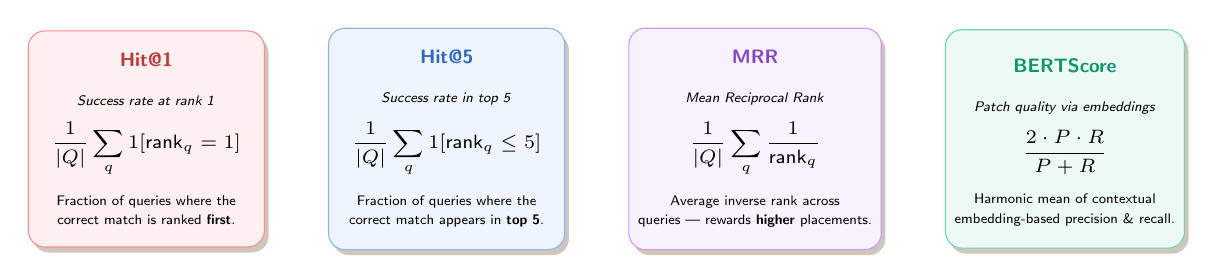
\begin{tikzpicture}[
    node distance=0.6cm and 1.2cm,
    mcard/.style={
      draw=#1!60, fill=#1!8,
      rounded corners=6pt,
      minimum width=3cm,
      minimum height=2.4cm,
      inner ysep=8pt,
      font=\scriptsize\sffamily,
      align=center,
      drop shadow={shadow xshift=1.5pt, shadow yshift=-2pt, opacity=0.3, fill=shadowcol}
    },
    mtitle/.style={
      font=\scriptsize\sffamily\bfseries,
      text=#1!80!black
    },
    micon/.style={
      font=\Large,
      text=#1
    }
  ]

    % --- Card 1: Hit@1 ---
    \node[mcard=ccode] (h1) {
      % \textcolor{ccode}{\faBuilding}\\[4pt]
      {\scriptsize\bfseries\textcolor{ccode!80!black}{Hit@1}}\\[6pt]
      {\tiny\textit{Success rate at rank 1}}\\[5pt]
      $\displaystyle\frac{1}{|Q|}\sum_{q} \mathbbm{1}[\text{rank}_q = 1]$\\[6pt]
      {\tiny Fraction of queries where the}\\[-1pt]
      {\tiny correct match is ranked \textbf{first}.}
    };

    % --- Card 2: Hit@5 ---
    \node[mcard=ccpg, right=0.8cm of h1] (h5) {
      % \textcolor{ccpg}{\faListOl}\\[4pt]
      {\scriptsize\bfseries\textcolor{ccpg!80!black}{Hit@5}}\\[6pt]
      {\tiny\textit{Success rate in top 5}}\\[5pt]
      $\displaystyle\frac{1}{|Q|}\sum_{q} \mathbbm{1}[\text{rank}_q \leq 5]$\\[6pt]
      {\tiny Fraction of queries where the}\\[-1pt]
      {\tiny correct match appears in \textbf{top 5}.}
    };

    % --- Card 3: MRR ---
    \node[mcard=cemb, right=0.8cm of h5] (mrr) {
      % \textcolor{cemb}{\faSortAmountDown}\\[4pt]
      {\scriptsize\bfseries\textcolor{cemb!80!black}{MRR}}\\[6pt]
      {\tiny\textit{Mean Reciprocal Rank}}\\[5pt]
      $\displaystyle\frac{1}{|Q|}\sum_{q} \frac{1}{\text{rank}_q}$\\[6pt]
      {\tiny Average inverse rank across}\\[-1pt]
      {\tiny queries — rewards \textbf{higher} placements.}
    };

    % --- Card 4: BERTScore ---
    
    
    \node[mcard=csub, right=0.8cm of mrr] (cwe) {
      \\[-0.5pt]
      {\scriptsize\bfseries\textcolor{csub!80!black}{BERTScore}}\\[6pt]
      {\tiny\textit{Patch quality via embeddings}}\\[5pt]
      $\displaystyle\frac{2 \cdot P \cdot R}{P + R}$\\[6pt]
      {\tiny Harmonic mean of contextual}\\[-1pt]
      {\tiny embedding-based precision \& recall.}
    };

  \end{tikzpicture}
  \end{center}
 

\end{frame}
% =====================================================================
% PHASE 1: AUTOPATCH RESULTS
% =====================================================================
\begin{frame}{ AutoPatch Dataset Results (n=225)}
  % \textbf{Goal:} Validate that structural embeddings match CodeBERT performance.

  \vspace{0.3cm}
  \begin{table}
    \centering
    \small
    \begin{tabular}{lrrrr}
      \toprule
      \textbf{Embedder} & \textbf{H@1} & \textbf{H@5} & \textbf{MRR} & \textbf{CWE R.} \\
      \midrule
      \multicolumn{5}{c}{\textit{Structure-Only}} \\
      \midrule
      \textbf{Combined} & \textbf{0.8904} & \textbf{0.9589} & \textbf{0.9162} & \textbf{0.4978} \\
      GIN & 0.7260 & 0.8767 & 0.7879 & 0.4427 \\
      WL & 0.6986 & 0.7945 & 0.7363 & 0.4386 \\
      \midrule
      \multicolumn{5}{c}{\textit{CodeBERT pretrained}} \\
      \midrule
      CodeBERT (baseline) & 0.1533 & 0.2200 & 0.1826 & 0.2933 \\
      CodeBERT (seq) & 0.7534 & 0.8630 & 0.7927 & 0.4121 \\
CodeBERT (pat) & 0.7123 & 0.8356 & 0.7677 & 0.4147 \\      \bottomrule
    \end{tabular}
    \\[2pt]
    {\tiny\textcolor{notecol}{Source: \texttt{experiments/output/checkpoint5/20260505\_141347\_experiment\_f59ab1/results.json}}}
  \end{table}

  
  \textbf{RQ1:} validated — structural \textit{graph} representations are \textit{effective} for vulnerability pattern retrieval in a synthetic dataset.
\end{frame}


\begin{frame}{AutoPatch Dataset: CWE Distribution}

  \begin{center}
    {\small\textbf{Distribution of CWE Types in the AutoPatch Dataset} {\scriptsize($N = 75$ real-world CVEs)}}\\[3pt]
    {\scriptsize
    \renewcommand{\arraystretch}{1.08}
    \setlength{\tabcolsep}{5pt}
    \begin{tabular}{llrrr}
      \toprule
      \textbf{CWE ID} & \textbf{Category Group} & \textbf{CWE Description} & \textbf{Count} & \textbf{Ratio (\%)} \\
      \midrule
      \rowcolor{hit!12}
      \textbf{CWE-20}  & Validation \& Logic & Improper Input Validation & \textbf{20} & \textbf{26.67\%} \\
      CWE-362 & Concurrency        & Race Condition / Synchronization & 16 & 21.33\% \\
      CWE-252 & Validation \& Logic & Unchecked Return Value & 12 & 16.00\% \\
      CWE-843 & Type Errors        & Type Confusion & 8  & 10.67\% \\
      CWE-416 & Memory Safety      & Use After Free & 6  & 8.00\% \\
      CWE-476 & Memory Safety      & NULL Pointer Dereference & 4  & 5.33\% \\
      CWE-703 & Validation \& Logic & Improper Handling of Exceptional Conditions & 3  & 4.00\% \\
      CWE-122 & Memory Safety      & Heap-based Buffer Overflow & 1  & 1.33\% \\
      CWE-125 & Memory Safety      & Out-of-bounds Read & 1  & 1.33\% \\
      CWE-787 & Memory Safety      & Out-of-bounds Write & 1  & 1.33\% \\
      CWE-400 & Resource Handling  & Uncontrolled Resource Consumption & 1  & 1.33\% \\
      CWE-754 & Validation \& Logic & Improper Check for Unusual Conditions & 1  & 1.33\% \\
      CWE-775 & Resource Handling  & Missing Release of Resource & 1  & 1.33\% \\
      \midrule
      \textbf{Total} & & & \textbf{75} & \textbf{100.00\%} \\
      \bottomrule
    \end{tabular}}
  \end{center}

  \vspace{0.25em}
  \begin{tcolorbox}[colback=hit!5, colframe=hit!70!black, boxrule=0.35pt,
    left=3pt, right=3pt, top=2pt, bottom=1pt, arc=2pt, width=\linewidth]
    \scriptsize
    The dataset is heavily weighted toward \textbf{Validation \& Logic} errors (49.3\%) and \textbf{Concurrency / Race Conditions} (21.3\%). The top three CWE types (\textbf{CWE-20}, \textbf{CWE-362}, and \textbf{CWE-252}) account for over \textbf{64\%} of all evaluated vulnerability instances.
  \end{tcolorbox}

  \vspace{0.15em}
  {\scriptsize\textcolor{notecol}{Source: \texttt{AutoPatch Benchmark Dataset ($N=75$)}}}

\end{frame}

% =====================================================================
% PHASE 2: CVEFIXES DATASET
% =====================================================================
\begin{frame}{\textbf{[OLD]}CVEfixes Dataset }
  
  \textbf{Question:} Does the approach generalize to real-world vulnerabilities?
  \vspace{0.3cm}
  
\begin{columns}[T]
\begin{column}{0.48\textwidth}

  \textbf{Real-World Dataset}\\[3pt]
  {\small CVEFixes datasets is large dataset with real-world CVEs collected from the U.S. National Vulnerability Database, patches, and code changes.\\}
  
  \vspace{0.5em}
  \begin{center}
    
  \scriptsize
  \begin{tabular}{lr}
    \toprule
    \textbf{Metric} & \textbf{Value} \\
    \midrule
    CVEs & 11,873 \\
    Fix commits & 12,107 \\
    File changes & 51,342 \\
    Method changes & 277,948 \\
    Repositories & 4,249 \\
    \bottomrule
  \end{tabular}
  \end{center}
\end{column}
\begin{column}{0.50\textwidth}
    {\small\textbf{Sampling criteria}}\\[3pt]
  {\scriptsize
  \begin{itemize}\itemsep1pt
      \setbeamertemplate{itemize item}{}
    \item Structurally distinshable CWEs (e.g. UAF vs. OOB) to test pattern matching, not just code similarity
    \item Balanced superclass(CWE) up to 20 entries and subclasses (CVE) to ensure retrieval feasibility
  \end{itemize}}
      \vspace{0.5em}
    \begin{center}
      {\scriptsize
  \renewcommand{\arraystretch}{1.2}
  \begin{tabular}{lr}
    \toprule
    \textbf{Parameter} & \textbf{Value} \\
    \midrule
    Total pairs & 136 \\
    Index set & 109 \\
    Query set & 27 \\
    Unique CVEs (index) & 60 \\
    Unique CVEs (query) & 25 \\
    CWE classes & 7 \\
    % Slice depth & 2-hop \\
    % Min/max lines & 10 / 120 \\
    \bottomrule
  \end{tabular}}
    \end{center}
  
\end{column}
\end{columns}
\end{frame}

\begin{frame}{\textbf{[NEW]} CVEfixes Dataset }
  
  \textbf{Question:} Does the approach generalize to real-world vulnerabilities?
  \vspace{0.3cm}
  
\begin{columns}[T]
\begin{column}{0.48\textwidth}

  \textbf{Real-World Dataset}\\[3pt]
  {\small CVEFixes datasets is large dataset with real-world CVEs collected from the U.S. National Vulnerability Database, patches, and code changes.\\}
  
  \vspace{0.5em}
  \begin{center}
    
  \scriptsize
  \begin{tabular}{lr}
    \toprule
    \textbf{Metric} & \textbf{Value} \\
    \midrule
    CVEs & 11,873 \\
    Fix commits & 12,107 \\
    File changes & 51,342 \\
    Method changes & 277,948 \\
    Repositories & 4,249 \\
    \bottomrule
  \end{tabular}
  \end{center}
\end{column}
\begin{column}{0.50\textwidth}
    {\small\textbf{Sampling criteria}}\\[3pt]
  {\scriptsize
  \begin{itemize}\itemsep1pt
      \setbeamertemplate{itemize item}{}
    \item Structurally distinshable CWEs (e.g. UAF vs. OOB) to test pattern matching, not just code similarity
    \item Balanced superclass(CWE) and at least 5 entries for each subclasse (CVE) to ensure retrieval feasibility
  \end{itemize}}
      \vspace{0.5em}
    \begin{center}

      {\scriptsize
      \renewcommand{\arraystretch}{1.2}
      \begin{tabular}{lr}
        \toprule
        \textbf{Parameter} & \textbf{Value} \\
          \midrule
            Total pairs & 450 \\
            Index set & 360 \\
            Test set & 90 \\
            Unique CVEs (index) & 26 \\
            Unique CVEs (query) & 25 \\
            CWE classes & 6 \\
          \bottomrule
      \end{tabular}}

    \end{center}
  
\end{column}
\end{columns}
\end{frame}

% =====================================================================
% FUNCTION VS. FILE
% =====================================================================

% \begin{frame}{\textbf{[OLD]} Balanced Dataset + Function Graph Input: Retrieval Results}
%   \begin{columns}[T]
%     \begin{column}{0.5\textwidth}

%   \begin{center}
%       {\small\textbf{Same-CWE Retrieval} {\scriptsize(n=109 index, 27 query)}}\\[6pt]
%         {\scriptsize
%         \renewcommand{\arraystretch}{1.35}
%         \setlength{\tabcolsep}{3.5pt}
%           \begin{tabular}{lrrrr}
%             \toprule
%             \textbf{Embedder} & \textbf{Hit@1} & \textbf{Hit@5} & \textbf{MRR} & \textbf{CWE Recall} \\
%             \midrule
%             GIN & 0.259 & 0.778 & 0.315 & 0.202 \\
%             \rowcolor{warn!12}
%             Combined & \cmiss{0.111} & 0.778 & 0.223 & 0.189 \\
%             CodeBERT (baseline) & 0.080 & 0.1518 & 0.098 & 0.141 \\
%             \rowcolor{hit!12}
%             \textbf{CodeBERT (seq)} & \textbf{0.556} & \textbf{0.926} & \textbf{0.555} & \textbf{0.264} \\
%             \textbf{CodeBERT (pat)} & \textbf{0.519} & \textbf{0.889} & \textbf{0.549} & \textbf{0.276} \\
%             \bottomrule
%           \end{tabular}
%         }

%         \vspace{0.3em}
%         {\tiny\textcolor{notecol}{Source: \texttt{cvefixes\_experiments/output/pipeline\_verification/results.json}}}
%     \end{center}
  
%   \end{column}
%  \begin{column}{0.5\textwidth}

%   \begin{center}
%   {\small\textbf{Per-CWE Breakdown} {\scriptsize(CodeBERT Pattern, CWE Hit@$k$)}}\\[6pt]
%   {\scriptsize
%   \renewcommand{\arraystretch}{1.35}
%   \setlength{\tabcolsep}{3.5pt}
%   \begin{tabular}{l r rrr}
%     \toprule
%     \textbf{CWE} & \textbf{N} & \textbf{Hit@1} & \textbf{Hit@5} & \textbf{Hit@10} \\
%     \midrule
%     Integer Overflow (190) & 4 & \chit{75\%} & 100\% & 100\% \\
%     Input Validation (20) & 4 & \chit{75\%} & 75\% & 100\% \\
%     Resource Consump.\ (400) & 3 & \chit{67\%} & 100\% & 100\% \\
%     Use After Free (416) & 4 & 50\% & 100\% & 100\% \\
%     NULL Ptr Deref (476) & 5 & \cwarn{40\%} & 80\% & 80\% \\
%     Race Condition (362) & 3 & \cwarn{33\%} & 100\% & 100\% \\
%     OOB Write (787) & 4 & \cmiss{25\%} & 75\% & 75\% \\
%     \midrule
%     \textbf{Overall} & \textbf{27} & \textbf{51.9\%} & \textbf{88.9\%} & \textbf{92.6\%} \\
%     \bottomrule
%   \end{tabular}}

%   \vspace{0.2em}
%   {\tiny\textcolor{notecol}{Source: same file (CodeBERT Pattern cell)}}

%   \vspace{0.2em}
%   {\scriptsize\textcolor{notecol}{Highlights areas for improvement in embedding design or slicing strategy.}}
%   \end{center}
%     \end{column}
%   \end{columns}
% \end{frame}


\begin{frame}{\textbf{[OLD]} Function vs. File: Same-Split Comparison}

  \begin{center}
    {\small\textbf{Function-level vs File-level Input} {\scriptsize(identical paired sample \& split: n=122 index, 37 query; seed 42; $G_{\mathrm{vuln}}$)}}\\[4pt]
  {\scriptsize
  \renewcommand{\arraystretch}{1.15}
  \setlength{\tabcolsep}{4pt}
    \begin{tabular}{llrrrrr}
      \toprule
      \textbf{Embedder} & \textbf{Input} & \textbf{Hit@1} & \textbf{Hit@5} & \textbf{Hit@10} & \textbf{MRR} & \textbf{CWE R.} \\
      \midrule
      GIN & function & 0.108 & 0.243 & 0.270 & 0.152 & 0.205 \\
      \rowcolor{miss!15}
      GIN & file & 0.081 & 0.189 & 0.216 & 0.122 & 0.145 \\
      \midrule
      Combined & function & 0.054 & 0.432 & 0.486 & 0.190 & 0.192 \\
      \rowcolor{hit!12}
      Combined & \textbf{file} & \textbf{0.622} & \textbf{0.649} & \textbf{0.730} & \textbf{0.642} & \textbf{0.255} \\
      \midrule
      CodeBERT (seq) & function & 0.351 & 0.595 & 0.730 & 0.451 & 0.249 \\
      \rowcolor{hit!12}
      \textbf{CodeBERT (seq)} & \textbf{file} & \textbf{0.811} & \textbf{0.865} & \textbf{0.919} & \textbf{0.845} & \textbf{0.281} \\
      \midrule
      CodeBERT (pat) & function & 0.351 & 0.649 & 0.784 & 0.463 & 0.264 \\
      \rowcolor{hit!12}
      CodeBERT (pat) & \textbf{file} & \textbf{0.757} & \textbf{0.811} & \textbf{0.865} & \textbf{0.785} & \textbf{0.289} \\
      \bottomrule
    \end{tabular}}
  \end{center}

  \vspace{0.35em}
  \begin{tcolorbox}[colback=hit!5, colframe=hit!70!black, boxrule=0.35pt,
    left=3pt, right=3pt, top=2pt, bottom=1pt, arc=2pt, width=\linewidth]
    \scriptsize
    On an \textbf{identical sample and split} (both levels share the same 122 index / 37
    query instances), file-level input strongly improves the semantic and fusion
    embedders --- Combined Hit@1 \textbf{+0.57}, CodeBERT (seq) Hit@1 \textbf{+0.46} /
    MRR \textbf{+0.39}, CodeBERT (pat) Hit@1 \textbf{+0.41}. The exception is
    \textbf{GIN} (pure topology, \textcolor{miss}{$-0.03$} Hit@1): the wider file context
    adds structure the semantic embedders exploit but that slightly dilutes GIN's
    topology-only signal.
  \end{tcolorbox}

  \vspace{0.2em}
  {\scriptsize\textcolor{notecol}{Source: \texttt{cvefixes\_experiments/output/method\_vs\_file\_level/comparison.json} (paired run, seed 42)}}

\end{frame}

\begin{frame}{\textbf{[NEW]} Function vs. File: Same-Split Comparison}

  \begin{center}
    {\small\textbf{Function-level vs File-level Input} {\scriptsize(identical paired sample \& split: n=122 index, 37 query; seed 42; $G_{\mathrm{vuln}}$)}}\\[4pt]
    {\scriptsize
    \renewcommand{\arraystretch}{1.15}
    \setlength{\tabcolsep}{4pt}
    \begin{tabular}{llrrrrr}
      \toprule
      \textbf{Embedder} & \textbf{Input} & \textbf{Hit@1} & \textbf{Hit@5} & \textbf{Hit@10} & \textbf{MRR} & \textbf{CWE R.} \\
      \midrule
      Combined & function & 0.333 & 0.656 & 0.811 & 0.454 & 0.384 \\
      \rowcolor{hit!12}
      Combined & \textbf{file} & \textbf{0.889} & \textbf{1.000} & \textbf{1.000} & \textbf{0.944} & \textbf{0.750} \\
      \midrule
      CodeBERT (seq) & function & 0.722 & 0.778 & 0.789 & 0.741 & \textbf{0.627} \\
      \rowcolor{hit!12}
      \textbf{CodeBERT (seq)} & \textbf{file} & \textbf{0.889} & \textbf{0.889} & \textbf{0.889} & \textbf{0.889} & 0.605 \\
      \midrule
      CodeBERT (pat) & function & 0.678 & 0.789 & 0.789 & 0.720 & 0.619 \\
      \rowcolor{hit!12}
      CodeBERT (pat) & \textbf{file} & \textbf{0.889} & \textbf{0.889} & \textbf{0.889} & \textbf{0.889} & \textbf{0.650} \\
      \bottomrule
    \end{tabular}}
  \end{center}

  \vspace{0.35em}
  \begin{tcolorbox}[colback=hit!5, colframe=hit!70!black, boxrule=0.35pt,
    left=3pt, right=3pt, top=2pt, bottom=1pt, arc=2pt, width=\linewidth]
    \scriptsize
    On an \textbf{identical sample and split}, shifting from function-level to file-level input consistently boosts performance across all models --- Combined Hit@1 \textbf{+0.556} / MRR \textbf{+0.490}, CodeBERT (seq) Hit@1 \textbf{+0.167}, CodeBERT (pat) Hit@1 \textbf{+0.211}. The only minor regression occurs in CodeBERT (seq) CWE Recall (\textcolor{miss}{$-0.022$}), while file context pushes Combined to perfect top-5/10 retrieval.
  \end{tcolorbox}

  \vspace{0.2em}
  % {\scriptsize\textcolor{notecol}{Source: \texttt{cvefixes\_experiments/output/method\_vs\_file\_level/comparison.json} (paired run, seed 42)}}

\end{frame}

\begin{frame}{\textbf{[NEW]} Patch Evaluation Across CWEs}

  \begin{center}
    {\small\textbf{Patch Evaluation Metrics Across CWEs} {\scriptsize(GPT-5.3-Codex, CodeBERT Sequence Embedder; $N=88$)}}\\[4pt]
    {\scriptsize
    \renewcommand{\arraystretch}{1.15}
    \setlength{\tabcolsep}{3pt}
    \begin{tabular}{lrrrrrrrr}
      \toprule
      \textbf{Category} & \textbf{Count} & \textbf{Exact Match} & \textbf{Hunk F1} & \textbf{BERTScore F1} & \textbf{BLEU-4} & \textbf{ROUGE-L} \\
      \midrule
      CWE-190 & 15 & 5 & 0.6149 & 0.6960 &  0.7504 & 0.7908 \\
      CWE-20  & 15 & 3 & 0.8643 & 0.9121 & 0.8579 & 0.9293 \\
      \rowcolor{hit!12}
      \textbf{CWE-362} & 15 & \textbf{8} & \textbf{0.9983} & \textbf{0.9648} & \textbf{0.9912} & \textbf{0.9961} \\
      CWE-416 & 14 & 10 & 0.9344 & 0.9387 & 0.9593 & 0.9730 \\
      CWE-476 & 14 & 9 & 0.9007 & 0.9334 & 0.8910 & 0.9246 \\
      \rowcolor{miss!15}
      CWE-787 & 15 & 0 & 0.2625 & 0.5243 & 0.8941 & 0.9431 \\
      \midrule
      \textbf{General (All)} & \textbf{88} & \textbf{35} & \textbf{0.7590} & \textbf{0.8258} & \textbf{0.8899} & \textbf{0.9256} \\
      \bottomrule
    \end{tabular}}
  \end{center}

  \vspace{0.35em}
  \begin{tcolorbox}[colback=hit!5, colframe=hit!70!black, boxrule=0.35pt,
    left=3pt, right=3pt, top=2pt, bottom=1pt, arc=2pt, width=\linewidth]
    \scriptsize
    Performance varies by vulnerability type: \textbf{CWE-362} (Race Conditions) achieves near-perfect fidelity (Hunk F1 \textbf{0.9983}, ROUGE-L \textbf{0.9961}), whereas \textbf{CWE-787} (Out-of-bounds Write) proves most challenging with 0 exact matches and a Hunk F1 of only \textcolor{miss}{\textbf{0.2625}}.
  \end{tcolorbox}

  \vspace{0.2em}
  {\scriptsize\textcolor{notecol}{Source: \texttt{cwe\_evaluation\_gpt5.3\_codebert\_seq.json}}}

\end{frame}

\begin{frame}{\textbf{[NEW]} Patch Evaluation Across CWEs (\texttt{CodeBERT\_seq} and GPT-4o)}

  \begin{center}
    {\small\textbf{Patch Evaluation Metrics Across CWEs} {\scriptsize($N=20$, Evaluated=$14$, Skipped=$6$)}}\\[4pt]
    {\scriptsize
    \renewcommand{\arraystretch}{1.15}
    \setlength{\tabcolsep}{4pt}
    \begin{tabular}{lrrrrrrrr}
      \toprule
      \textbf{Category} & \textbf{Total} & \textbf{Evaluated} & \textbf{Skipped} & \textbf{Exact Match} & \textbf{Hunk F1} & \textbf{BERTScore F1} & \textbf{BLEU-4} & \textbf{ROUGE-L} \\
      \midrule
      \rowcolor{hit!12}
      \textbf{CWE-362} & 11 & 11 & 0 & \textbf{4} & \textbf{0.9553} & 0.4771 & 0.4528 & 0.4889 \\
      CWE-476          & 3  & 3  & 0 & 1          & 0.3333          & \textbf{0.6983} & \textbf{0.7506} & \textbf{0.7931} \\
      \rowcolor{miss!15}
      \textbf{Skipped/Unchecked} & 6 & 0 & \textcolor{miss}{\textbf{6}} & -- & -- & -- & -- & -- \\
      \midrule
      \textbf{General (All)} & \textbf{20} & \textbf{14} & \textcolor{miss}{\textbf{6}} & \textbf{5} & \textbf{0.8220} & \textbf{0.5245} & \textbf{0.5166} & \textbf{0.5541} \\
      \bottomrule
    \end{tabular}}
  \end{center}

  \vspace{0.35em}
  \begin{tcolorbox}[colback=miss!5, colframe=miss!70!black, boxrule=0.35pt,
    left=3pt, right=3pt, top=2pt, bottom=1pt, arc=2pt, width=\linewidth]
    \scriptsize
    \textbf{Evaluation Scope \& Skipping:} Out of $20$ total records, \textcolor{miss}{\textbf{6 entries (30\%) were skipped}} prior to evaluation. Across the $14$ evaluated records, \textbf{CWE-362} leads in Hunk F1 (\textbf{0.9553}) and exact matches ($4/11$), whereas \textbf{CWE-476} achieves higher standard semantic similarity scores (BLEU-4 \textbf{0.7506}, ROUGE-L \textbf{0.7931}).
  \end{tcolorbox}

  \vspace{0.2em}
  % {\scriptsize\textcolor{notecol}{Source: \texttt{evaluation\_results.json}}}

\end{frame}

% ── closing ───────────────────────────────────────────────────────────
\begin{frame}[plain]
\centering
\vspace{3em}
{\LARGE\bfseries\color{c1} Questions?}\\[2em]

\begin{tikzpicture}
  \node[draw=c1!30, rounded corners=6pt, fill=c1!5,
        minimum width=9cm, minimum height=1.4cm,
        font=\small\sffamily\color{notecol}, align=center]
    {Lívia Cavalcanti\quad\textbar\quad\faIcon{github}\ \texttt{graph-rag/}};
\end{tikzpicture}
\end{frame}

\end{document}

